\chapter{Procedure}
\section{Setup}
The experiment uses a transparent cryostat, a double-walled piece of glassware that is evacuated during the experiment, shown in \autoref{fig:cryostat}.
The probe chamber is located at the end of an elongated section of the cryostat and sits between the poles of a magnetic yoke.
The cryostat is cooled with liquid nitrogen, which is held in a toroidal storage tank.
The probe chamber is connected to the storage tank via a small tube, the flow of liquid nitrogen is limited by the static pressure due to nitrogen evaporating in the probe chamber.
Venting the probe chamber with the topmost valve regulates the pressure and in turn the flow of liquid nitrogen.

A heating coil, which is regulated by a PID controller, is used to accurately set the temperature of the probe chamber.
This gives a total temperature range of \SIrange{-180}{150}{\celsius} for the experiment.

\begin{figure}
	\centering
	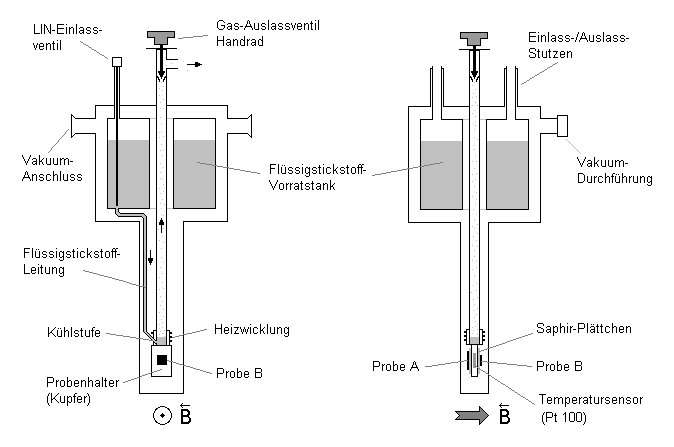
\includegraphics[width=.7\textwidth]{./img/cryostat.png}i
	\caption[Cryostat]{\textbf{The cryostat} used in the experiment}
	\label{fig:cryostat}
\end{figure}

\section{Samples}
\subsection{Sample A (Ge)}
Sample A is a block of germanium of dimensions \SI{19}{\mm} x \SI{10}{\mm} x \SI{1}{\mm}.
Contacts are made with thin gold wires, which are attached to electrolytically gold plated areas of the sample.
The exact geometry is shown in \autoref{fig:samples:ge}.

\subsection{Sample B (GaAs 2DEG)}
Sample B is a 2D electron gas inside a GaAs heterostructure.
The individual layers are depicted in the cross section \autoref{fig:samples:gaas-cross}.
The 2DEG forms between the active GaAs layer and the n-doped layer of AlGaAs.
The macroscopic shape of the sample is shown in \autoref{fig:samples:gaas-clover}.
The clover leaf or cross shaped geometry is chosen to minimize errors introduced by effects of the imperfect metal-semiconductor contact, as discussed in \autoref{sec:van-der-pauw-geometry}.

The electron density $n_\text{2D}$ and mobility $\mu$, as stated by the manufacturer, are listed in \autoref{tab:lit-2deg}

\begin{table}
	\centering
	\captiond{Parameters of the 2DEG}{(stated by the manufacturer)}
	\label{tab:lit-2deg}
	\begin{tabular}{SSS}
		\toprule
		{$T$ (\si{\kelvin})}&	{$n_\text{2D}$ (\si{\per\centi\meter\squared})}&	{$\mu$ (\si{\centi\meter\squared\per\volt\per\second})}\\
		\midrule
		300&	2.9e11&	6.5e2\\
		70&	1.7e11&	1.94e5\\
		\bottomrule
	\end{tabular}
\end{table}

\begin{figure}
	\centering
	\begin{subfigure}{0.45\textwidth}
		\centering
		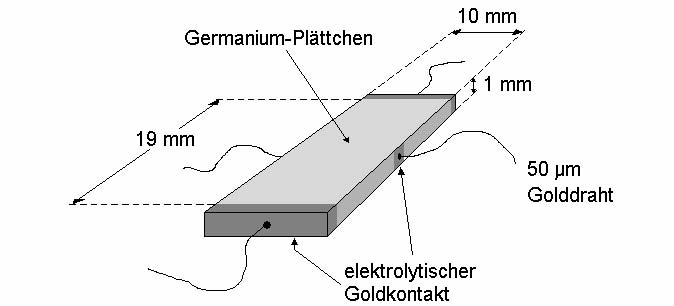
\includegraphics[width=\textwidth]{./img/sample-ge.png}
		\caption{Sample A (Ge)}
		\label{fig:samples:ge}
	\end{subfigure}
	\begin{subfigure}{0.45\textwidth}
		\centering
		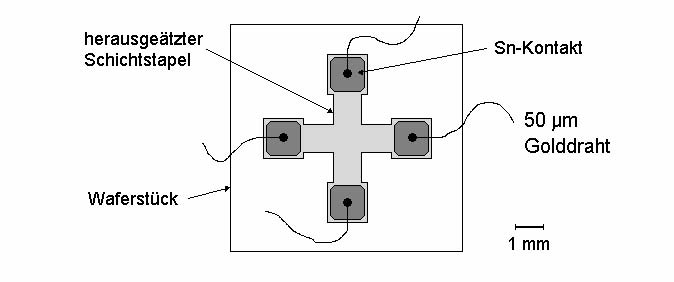
\includegraphics[width=\textwidth]{./img/sample-gaas-clover.png}
		\caption{Sample B (GaAs)}
		\label{fig:samples:gaas-clover}
	\end{subfigure}
	\begin{subfigure}{0.7\textwidth}
		\centering
		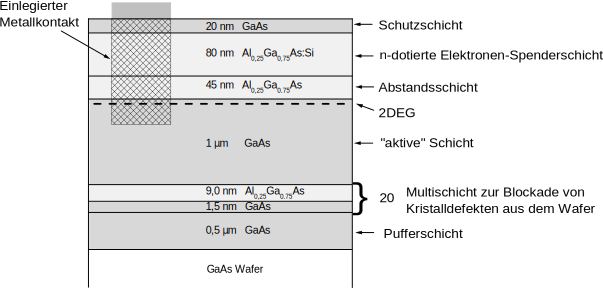
\includegraphics[width=\textwidth]{./img/sample-gaas-cross.pdf}
		\caption{Sample B (GaAs) cross section}
		\label{fig:samples:gaas-cross}
	\end{subfigure}
	\captiond{The samples}{used in the experiment}
\end{figure}
